\section{Application Examples}

\subsection{Identification of minor oxides}


    \renewcommand{\coef}{0.45}
    \begin{figure}[h]
        \centering
        \begin{subfigure}{\coef\textwidth}
            \centering
            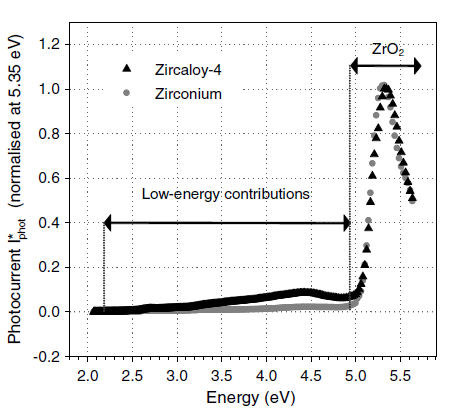
\includegraphics[width=\textwidth]{./src/figures/Benaboud2007-Fig4.png}
            \caption{}
            \label{fig:benaboud_minor_oxides_a}
        \end{subfigure}
        \begin{subfigure}{\coef\textwidth}
            \centering
            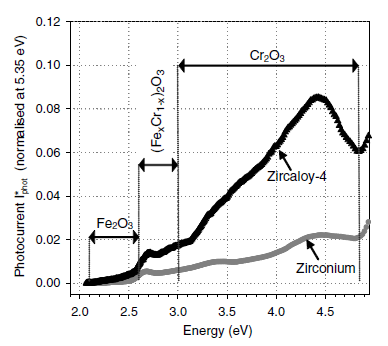
\includegraphics[width=\textwidth]{./src/figures/Benaboud2007-Fig5.png}
            \caption{}
            \label{fig:benaboud_minor_oxides_b}
        \end{subfigure}
        
        \caption{Photocurrent spectra measured on zirconia oxide layer formed on 
        Zircaloy4 and “pure” zirconium oxidized for 1h at 470°C in oxygenated 
        atmosphere\citep{benaboud2007}: a) complete spectrum b) close-up view on the minor contributions.}
        \label{fig:benaboud_minor_oxides}
    \end{figure}



\subsection{Identification of semiconduction type}

    \renewcommand{\coef}{0.45}
    \begin{figure}[h]
        \centering
        \begin{subfigure}{\coef\textwidth}
            \centering
            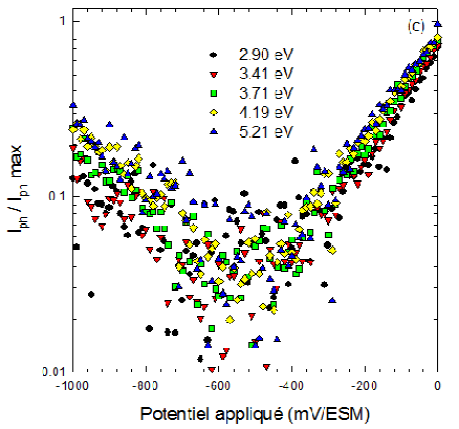
\includegraphics[width=\textwidth]{./src/figures/Loucif2012-Fig3-18.png}
            \caption{}
            \label{fig:loucif_sctype_a}
        \end{subfigure}
        \begin{subfigure}{\coef\textwidth}
            \centering
            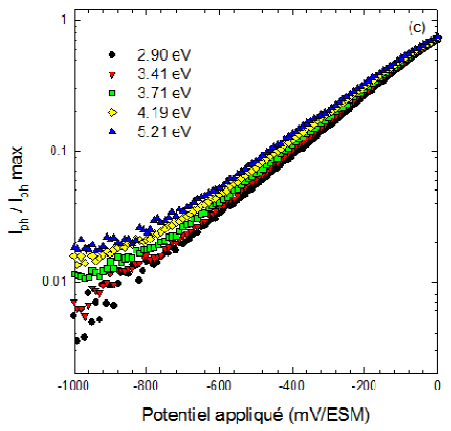
\includegraphics[width=\textwidth]{./src/figures/Loucif2012-Fig3-19.png}
            \caption{}
            \label{fig:loucif_sctype_b}
        \end{subfigure}
        
        \caption{Photocurrent with respect to the potential for an 
        Ni-based alloy 600 polished and oxidized in simulated PWR 
        for 500~h \citep{loucif2013}: a) $P_{H_2}$=6.5~bar, b) $P_{H_2}$=0.05~bar.}
        \label{fig:loucif_sctype}
    \end{figure}



\subsection{High temperature PEC}


    \renewcommand{\coef}{0.45}
    \begin{figure}[h]
        \centering
        \begin{subfigure}{\coef\textwidth}
            \centering
            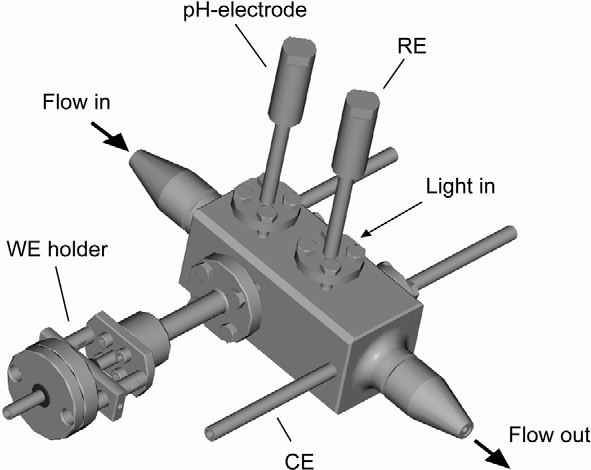
\includegraphics[width=\textwidth]{./src/figures/Bojinov_2002_Fig1.png}
            \caption{}
            \label{fig:bojinov_ht_a}
        \end{subfigure}
        \begin{subfigure}{\coef\textwidth}
            \centering
            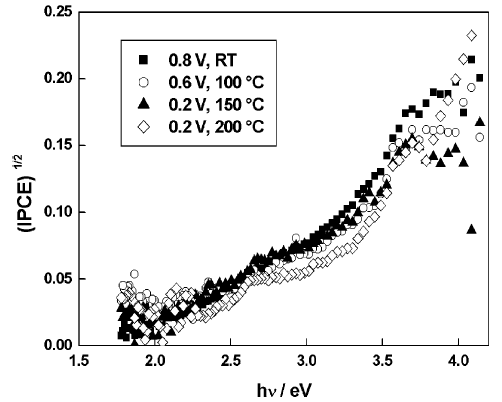
\includegraphics[width=\textwidth]{./src/figures/Bojinov_2002_Fig5b.png}
            \caption{}
            \label{fig:bojinov_ht_b}
        \end{subfigure}
        
        \caption{a) Schematic representation of the metallic cell developed
        by \citet{bojinov2002}. 
        b) Photocurrent spectra performed on iron oxides at different 
        temperatures (up to 200°C) obtained by \citet{bojinov2002}.}
        \label{fig:bojinov_ht}
    \end{figure}



    \renewcommand{\coef}{0.45}
    \begin{figure}[h]
        \centering
        \begin{subfigure}{\coef\textwidth}
            \centering
            \includegraphics[width=\textwidth]{./src/figures/skocic2015-1.png}
            \caption{}
            \label{fig:skocic_phd_cell}
        \end{subfigure}
        \begin{subfigure}{\coef\textwidth}
            \centering
            \includegraphics[width=\textwidth]{./src/figures/skocic2015-2.png}
            \caption{}
            \label{fig:skocic_phd_htpec}
        \end{subfigure}
        
        \caption{a) Schematic view of the photoelectrochemical cell developed by \citet{skocic2016}. 
        b) Photocurrent energy spectra of an X750 specimen recorded at room
        temperature and in 280°C/80 bar water \citep{skocic2016}}
        \label{fig:skocic_phd}
    \end{figure}
